

\documentclass{article}
\title{CSC3095:Web Platform for Digital Deployment of Virtual Servers}

\date{03.03.2017}
\author{Plamen Kolev\\ \textbf{Student number} : 130221960\\ \textbf{Supervisor} : Neil Speirs}

% USERPACKAGES
\usepackage{hyperref}

\usepackage{graphicx}
\graphicspath{ {resources/images/} }
\usepackage{glossaries}
\usepackage{cite}
\usepackage{color}
\usepackage[english]{babel}
\usepackage{filecontents}
\usepackage[dvipsnames]{xcolor}
\usepackage[numbers,sort&compress]{natbib}
\usepackage{ifthen}
\usepackage{pdfpages}
\usepackage{listings}

% ENDUSERPACKAGES

% CUSTOM MACROS

\makeglossaries
\let\oldcite=\cite
\renewcommand\cite[1]{\ifthenelse{\equal{#1}{_NEEDED_}}{[citation~needed]}{\oldcite{#1}}}
\renewcommand*{\glstextformat}[1]{\textcolor{blue}{#1}}
% ENDCUSTOMMACROS

\definecolor{Mycolor2}{HTML}{4a4a4a}
\hypersetup{
    colorlinks,
    citecolor=blue,
    filecolor=blue,
    linkcolor=Mycolor2,
    urlcolor=blue
}


	\newglossaryentry{bash}
{
	name=bash,
	description={Bourne Again SHell, a UNIX command line virtual shell language}
}

\newglossaryentry{open-source}
{
	name={open-source},
	description={Software that makes its code openly available, allows derived work without restrictions and its distribution is done freely}
}

\newglossaryentry{operating-system}
{
	name={operating system},
	description={The platform on which all user and system software is running. Examples are Windows, Linux, OSX, Android, iOSX}
}

\newglossaryentry{ssh}{
	name={ssh},
	description={
		SSH: secure shell, a network protocol that allows a remote connection to a terminal
	}
}

\newglossaryentry{natnetwork}{
	name={NAT network},
	description={
		A technique where one IP address is mapped to more internal ip addresses, used for security and reduced number of ips. \cite{whatisnat}
	}
}

\newglossaryentry{ipaddress}{
	name={IP address},
	description={
		An identifier that helps locating a resource on the network, usually represents a computer device connected to a network (local or )
	}
}

\newglossaryentry{api}{
	name={API},
	description = {
		Application Programmable interface, usually a way for exposing features of a certain program to the developer. Often used to automate a task.
	}
}

\newglossaryentry{vagrant}{
	name={Vagrant},
	description = {
		Vagrant provides easy to configure, reproducible, and portable work environments built on top of industry-standard technology and controlled by a single consistent workflow to help maximize the productivity and flexibility of you and your team. \cite{vagrant-definition}
	}
}

\newglossaryentry{puppet}{
	name={puppet},
	description={
		Open source Puppet helps you describe machine configurations in a declarative language, bring machines to a desired state, and keep them there through automation.\cite{puppet-definition}
	}
}

\newglossaryentry{ruby-on-rails}{
	name={Ruby On Rails},
	description={
		Rails is a web application development framework written in the Ruby language. It is designed to make programming web applications easier by making assumptions about what every developer needs to get started. It allows you to write less code while accomplishing more than many other languages and frameworks.\cite{ruby-on-rails-definition}
	}
}

\newglossaryentry{ruby}{
	name={ruby},
	description={
		A dynamic, open source programming language with a focus on simplicity and productivity. It has an elegant syntax that is natural to read and easy to write.\cite{ruby-definition}
	}
}

\newglossaryentry{html}{
	name={html},
	description={
		Hypertext Markup Language, used for displaying web page
	}
}


\begin{document}
\pagenumbering{gobble}
\maketitle

\newpage
\section{Declaration}
I declare that this dissertation represents my own work except where otherwise stated.

\section{Acknowledgements}


\newpage
\section{Abstract}

\newpage
\tableofcontents
\newpage
\listoffigures
\newpage
\pagenumbering{arabic}

\newpage
\section{Introduction}

As of the year 2016, there are currently three billion people that have access to the internet \cite{ictonline}. Google handles between two and three billion search queries per day \cite{a}. Dealing with so many requests on daily basis requires full utilisation of the available hardware in terms of resources. Part of Google's ability to scale and be efficient is due to the emergence of cloud infrastructure. The topic of the paper deals  with one of the building blocks of cloud computing, which is virtualisation.

\begin{quote}
	"The quickest and cheapest method to providing the necessary level of abstraction in terms of server resource is currently virtualisation\ldots" \par\raggedleft--- \textup{Paul Robinson}, Google Cloud Computing \cite{SecuringtheCloud}
\end{quote}


The term virtualisation is defined as the ability of one piece of hardware to run multiple operating systems \cite{b}. In this paper, a virtual machine, or an instance, is an operating system that runs on top of a "physical" operating system. The "physical" \gls{operating-system} is often referred to as the "host" system. Creating a platform that uses such technology enables an organisation to quickly set up any environment (operating system) that can be used in a variety of cases.

A company that wants to buy a high performing computer for each employee would requires physical access to perform repairs and maintenance and management. Physical systems are also more difficult to manage due to their non-central distribution. Another downside is non-scalable hardware utilisation, a case where one machine uses maximum resources but another one is idle. These are some problems that virtualisation technology can deal with.  It is now a core part of most new desktop Intel© processors and is integral part of all server-grade processors.

This helps with performance, as a virtual machine can be configured on the fly to use flexible amount of resources or even use shared pool of computational units. This technology also allows for easy server migration. A physical machine cannot be moved within couple of minutes to a different continent, whereas a virtualised operating system can be copy-pasted at will for very little cost. Physical infrastructure is also prone to hardware-related bugs. This is a case when a distributed software solution causes issues, because it was not tested on all the machines that run it.

How does virtualisation allow for easy \gls{migrations}? It achieves its task by abstracting away the available physical hard drives. On the virtualised host, they appear as a large pool of \gls{partitions} with the data ready for access. Having access to the virtualisation host allows the content of such system to be copied all at once to a different provider with the only requirement - have enough capacity to store the information. The alternative without using a virtualisation platform would be to gain physical access to each hard drive individually and copying the data incrementally.

\texttt{add more domain specific information}

\subsection{Purpose}
The project aims to utilise open-source virtualisation technology and make the process of managing and creating virtual machines automated through a web interface. A system manager should be able to open a website, fill in a web form with enough information about the desired \gls{operating-system}, click a button and create it.

The manager should also be able to obtain and generate credentials for that machine, as well as mark common packages for installation on it. The solution should also show performance statistics and allow for network port management. These features, alongside the benefits of virtualisation should create a strong and secure infrastructure for many applications, from virtual office workstation, to server testing and deployment.

# Expand on each of the examples

\texttt{Strong cryptography, virtual guest isolation, firewall rules, credential and authentication methodologies will be explored and will be the pillars of the system's security.}
\subsection{Aim and Objectives}
\subsubsection{Aim}
Give developers a platform for easy deployment, management and monitoring of virtual servers
\subsubsection{Objectives}

\begin{enumerate}
	\item Deploy a virtual machine of the user's choice through shell scripts
	      \begin{itemize}
		      \item The main feature of the solution is the deployment of the virtual machine instances. The following will be achieved by using Oracle's virtualisation documentation for Virtualbox and the shell scripting language and the automation tool puppet.
	      \end{itemize}

	\item Configure firewall settings
	      \begin{itemize}
		      \item Will be achieved through the virtualisation technology's API. The purpouse is toadd extra security layer to the guest \gls{operating-system}. The firewall settings are managed by a software called ufw - Uncomplicated FireWall
	      \end{itemize}

	\item Allow console access and set up authentication credentials (SSH keys) for the instances
	      \begin{itemize}
		      \item The main usage of the application is to obtain a shell access to the virtual machine
	      \end{itemize}
	\item Monitor disk/CPU usage of the virtual instances
	\item Allow the user to install software from a predefined list
	\item Create a website that will manage and create the machines on the behalf of the user
\end{enumerate}

\newpage
\section{Background}
\subsection{Virtualisation}
\subsection{Addoption}
\subsection{Application}
\newpage
\section{Planning}

\begin{center}
	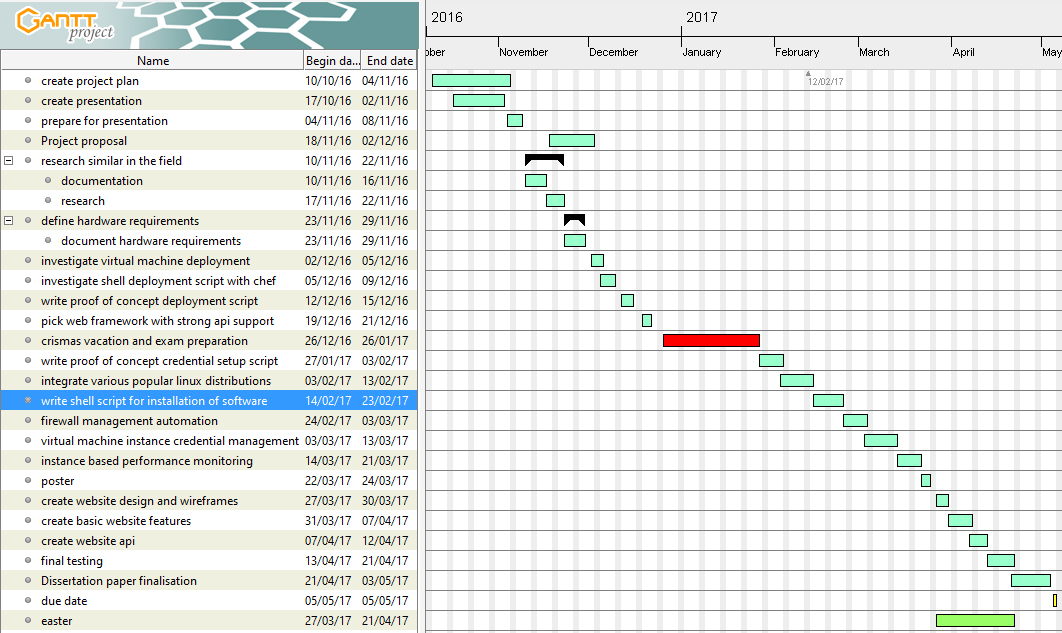
\includegraphics[width=12cm]{gantt.jpg}
\end{center}

As part of the development cycle, I have scheduled a meeting every fortnight with my supervisor to discuss work progress. During these meetings, I received feedback, raised concerns and showed progress in a \gls{standup} fashion. Occasionally, the meetings were not about progress update, but about demonstration of the work done so far with the purpose of obtaining feedback.

\subsection{First Semester}
When creating the project plan, two core stages were taken into consideration. The first stage is semester one. During that period, the ground work was laid, on which all future development and testing work was based. This is a critical moment into the building process. It allowed for a more in-depth research using materials created by the leading experts in the field (Amazon, Intel, Oracle). These documents helped gaining more understanding in various aspects of building cloud-ready applications, infrastructure security and automation.

The research helped when rationing about the features that need implementing. It also illustrated the scope, and the challenges that need to be faced. The research gave an insight into why this problem requires solving, and pointed me to open-source projects that achieve parts of the work.

The first semester was not only about research, but also about describing the constrains, limitations and infrastructure decisions that need to be made in order to demonstrate a  product that has real-world applications.
The materials helped me also to identify potential risks and issues that might arise, such as the security risk of running multiple virtual machines onto the same physical space. This is a potential risk situation, as an attacker can read the private data of another machine if the person gets access to the memory of the "host".

Work also went into creating presentation and project proposal for the upcoming work, which give an outline and highlighted the features that the work addresses.
When creating the presentation, I wanted to be as generic as possible as not to present information and ideas that the additional research might prove impossible to implement or not practical.

\subsection{Second Semester}

The tasks accomplished during the second semester are related to implementing, refining, iterating, evaluating and documenting the solution. This is the time where all the main features, functional and non-functional requirements got developed, tested and documented. It must be noted that for the most part, each cycle was not incrementally tackled, but instead, numerous development-testing-documenting phases were used to achieve the final result.
\begin{center}
	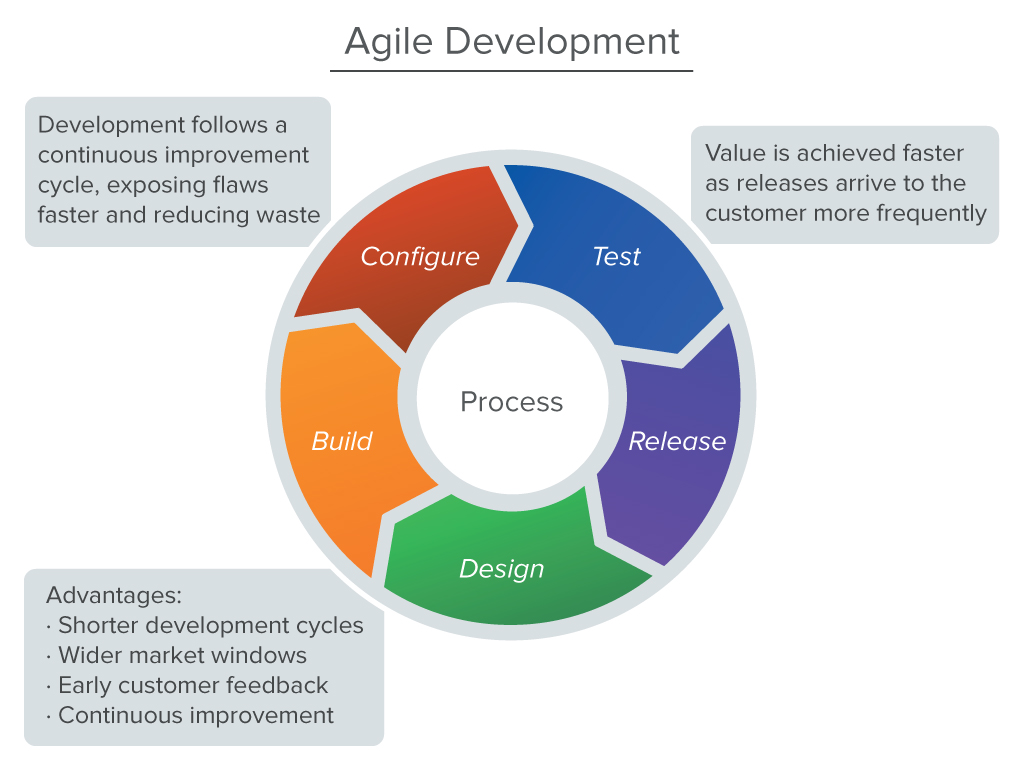
\includegraphics[width=12cm]{agile.jpg}
\end{center}

For the most part, the project was completed using the agile methodology. Each cycle that shaped the final product is described below.
\subsubsection{Developmen}
As planned, I broke down the main objectives into subtasks and tackled them one-by-one. My initial plan is not to develop the whole system and assemble the parts together at the end, but to build a minimum viable product (MVP) and increment onwards.

This was done in order to assure that the platform can be built with the available tools and that the requirements can be met at the end of the project.

Being able to create a virtual machine with a known \gls{ipaddress} from a script was the first thing that had to be accomplished. Creating custom users, opening ports and creating the web interface was planned later as something that could be built on top of the "core" product.

\subsubsection{Learning period}
For the duration of this project, a variety of new technologies were tried and evaluated, such as \gls{vagrant}, \gls{puppet}, \gls{ruby-on-rails}, \gls{ruby}.

As part of the learning cycle, the official ruby programming language manual was used. It helped gain proficiency to understand the fundamental constructs that were used throughout the tutorials, articles, blogs and other learning materials. The process taught me about declaring variables, scopes, for loops and any extra syntax unlike other programming languages. To get up and running with \gls{ruby}, the period between first and second semester was planned to build basic command line programs.

Another part of the development strategy was to do a small web project using ruby on rails just to get a feeling of what is possible in terms of rapid development and ease of use. This small project included building forms, validation, manipulating database objects and creating \gls{html} pages. This was done in February (the beginning of second semester), with the purpose of determining if this tool is right for the job

The task of learning \gls{puppet} was achieved by creating end-to-end automation scrip of the current set-up of my desktop machine. Puppet's power is to get a machine's configuration to a known state and ensure all software packages are present. Doing this exercise was overall a good practice, as it led to a faster implementation and integration later on when working on the actual platform.

\subsubsection{Documentation}
The initial plan as stated in the project proposal is to document the work during each stage of the process. 



\newpage
\section{Methodology}
\subsection{Overview}
This chapter aims to give a more in-depth view into the process of scoping, developing, planning and building the application. This ranges from picking the tools to limiting the scope, making assumptions, as well as the scheduling of each task. Creating such a platform from nothing is a daunting task even for an experienced senior software engineer.

For the above reason, the initial research into building the right tool-chain was essential to the success of the project.

The development methodology can be broken into the following steps:
\begin{enumerate}
	\item
	      Research into virtualisation technology to understand the underlying architecture.

	\item
	      Select free and open-source software components that can be coupled together to orchestrate and utilise above mentioned technology. The public libraries used also allowed me to extend, modify and build on top of during the development process.

	\item
	      Build a set of core and advanced features. Core features are essential for a good operational and usable solution. Advanced features are the things that make this solution go above and beyond the scope of existing applications.

	\item
	      Integrate components into one final solution

	\item
	      Do sufficient testing to ensure that the platform behaves as expected.
\end{enumerate}

\subsection{Similar in the field}
For the duration of my dissertation, I have evaluated a variety of technologies, frameworks and utilities that will allow me to achieve the goal of automated system deployment. The trial and evaluation of these technologies allowed me to find the most suitable and relevant methodology for moving forward. I also experimented with different "cloud" virtual machine deployment services to understand and evaluate the key requirements that ought to be provided by the platform that I am building.

\subsection{Constrains}
Because of the limited duration of the dissertation and the immense work that has to be carried throughout the implementation (testing, documentation, development, debugging, planning, etc.) certain constrains had to be put in place to ensure that the project will be completed within the appropriate period.

The initial constrain that I have defined is limiting the solution to a single host. This work is done as a proof-of-concept system that has the potential of being scaled up and extended to support "real-world" application.
Creating a distributed and scalable implementation of this work goes beyond the scope. This is not to say that it is limited to single host, but testing and planning guarantee that it will be fully functional under such condition.

As a future task, it would be possible to deploy multiple instances of the underlying infrastructure that are managed and synchronised with a technology like puppet or chef. Then, creating virtual machines can be done via a manager machine that picks a host based on a round-robin algorithm or based on load. Additional implementation steps must be carried out to ensure that the web platform and the manager understands the physical location of the virtual machine. Physical location references to the real hardware (the host) running the virtual machine.

Another assumption and a constrain is the availability of a network interface. To simplify the development process and allow me to isolate different environments. A network environment is the space in which all the virtual machines have visibility of one another. It also makes it possible to allocate different network addresses dynamically and verify availability of resources. Another important bit is the fact that one must be connected to the network environment to communicate with the machines inside of it. I have taken advantage of VirtualBox's host-only networking interfaces, and have created multiple instances that allow me to create machines independent of each other when developing and testing.

When further extending the solution, additional work has to be carried out to ensure integration with a public DNS server, and some adjustments ought to be made to allow the production DNS to allocate \textcolor{red}{DHCP} ip addresses to the virtual machines.

The solution aims to orchestrate and automate generic virtual machine deployment, but creating a solution that enables every \gls{operating-system} to be deployable would require extensive amount of extra work. Future work can make it possible to deploy Windows, Mac OS and more Linux variants as part of the infrastructure, but this is yet not the case.

Windows is not supported yet, as it has completely different architecture and has a separate interface for managing networking, users, installation and permissions. Doing windows deployment also requires licensing of their \gls{operating-system}. Another constrain in working with windows is that not many core components are configurable or accessible via a script making automation very difficult or impossible.

Mac OSX virtual deployment was also something left for future. It also has similar issues to windows virtualisation (licensing, exposed \gls{api}).

Finally, as it comes to Linux virtual machine deployment, I have opted to cover

\subsection{Functional requirements}
\subsection{Non-functional requirements}
\subsection{Tools}

\section{Development}
A hypervisor is a computer software or hardware that creates the platform layer to a virtual machine and makes it possible to host multiple instances with different configurations \cite{ibmvirtualisation}.

Initially, I was planning on using a hypervisor virtualisation solution such as Virtualbox and VMware, and use the \gls{bash} shell scripting language to interface directly with them. With this in mind, I decided to opt for Virtualbox, as it is an \gls{open-source} software solution, has strong community, allows third party plug-ins There are other alternatives (gnome boxes, CHROOT), but what draw me to it is that it is configurable and command-line controllable straight out of the box. Another deciding factor was also the extensibility that is offered by third party modules developed by the community.

Another reason for not choosing a more unpopular or niche technology is due to the willingness of an adopter to switch their entire virtual infrastructure to it. The Virtualbox software is very popular, and as such, it would make the transition much more subtle and unnoticeable

As part of my research, I went through the Virtualbox command-line API. In the process of doing so, I discovered the variety of customisable parameters when building a virtual machine, like the different possibilities in setting up networks (private, network shared, host only, etc.), exposing ports, as well as different hardware configurations (RAM, hard drive, CPU count). After using the command line tools and writing a simple shell scripts for managing creation of different resources, I realised that a tool needs to be written to manage the different technical details of each virtual machine. Luckily, an open-source hypervisor provisioner software is available that helps with automation and management that satisfies the operational needs of the system.

\subsection{Vagrant}
The tool is called Vagrant by Hashicorp, a company specialising in easy virtual machine configuration management and set-up Their API provides the following features.

\begin{itemize}
	\item
	      Allow the administrator to create a \gls{vagrant} configuration file (called Vagrantfile), which describes end-to-end each operation that will be performed to the virtual machine instance (including the Linux distribution that will get installed on it).
	\item
	      Create a system compatible with their platform starting from a bare configuration and incrementally building a bespoke instance. These instances can be managed and shared on the internet.
	\item
	      Managing network interfaces
	\item
	      Configure ports
	\item
	      Allow \gls{ssh} access
\end{itemize}

\subsection{Architecture}
When considering the architecture of the system, a list of factors were the driving factor when building the solution. I wanted to ensure that The solution has as little moving parts as possible, which will allow it to be flexible and extensible. For that purpose I chose the programming language \gls{ruby}, as it is a suitable language for system automation. Its suitability comes from the available tools \gls{vagrant} and \gls{puppet} which allow end-to end integration when it comes to automation. The \gls{ruby} programming language also draws inspiration from the Perl programming language One of the Perl's strengths is its ability to be a more powerful shell scripting language. This is the case as it has quick syntax for executing shell scripts directly and get STDOUT, STDERR and exit-codes quickly. It does also has native implementation of common UNIX tools, like grep, wget and awk.

Because the Ruby language draws inspiration and shares similar features with Perl, it makes it a great modern and powerful language to use in this domain-specific problem.

The framework I created uses a virtual machine instance object and authenticated user that owns it. When the user fills the web form with the relevant information, it will pass the configuration values directly to a virtual machine class. This class contains a dynamic configuration, which ensures that the solution is distribution agnostic. Here, the term distribution references to the different versions of Linux (ubuntu, fedora, Centos, arch Linux). Separating dependency specific configuration by sub-classing a configuration object allows for a quick way for the project to be extended to accommodate for new distributions.

For the purpose of this work, I have decided to limit the scope of allowed Linux distributions to Ubuntu, Centos and debian, but it is important to note that the architecture allows extending that list.

To do so, folder with the name of the new distribution must be placed in lib/configurations that describes the configuration specific settings that include updating and installing common software packages.

The framework also uses UNIX environmental variable to manage infrastructure state. For the  purpose of developing and testing, I have created two main isolated environments - testing and development.
The most notable usage of such environment is the virtual host-only network that ensures that the virtual interfaces do not clash during testing and development. The two interfaces are \texttt{vboxnet0} and \texttt{vboxnet1}. One is for general purpose development, the another is for testing. A special host-only adapter is used to have an isolated ip range that is network agnostic, for example, on a \gls{natnetwork}, some IP addresses might be reserved or used, this case will cause a clash and the virtual machine will not be reachable.

\newpage
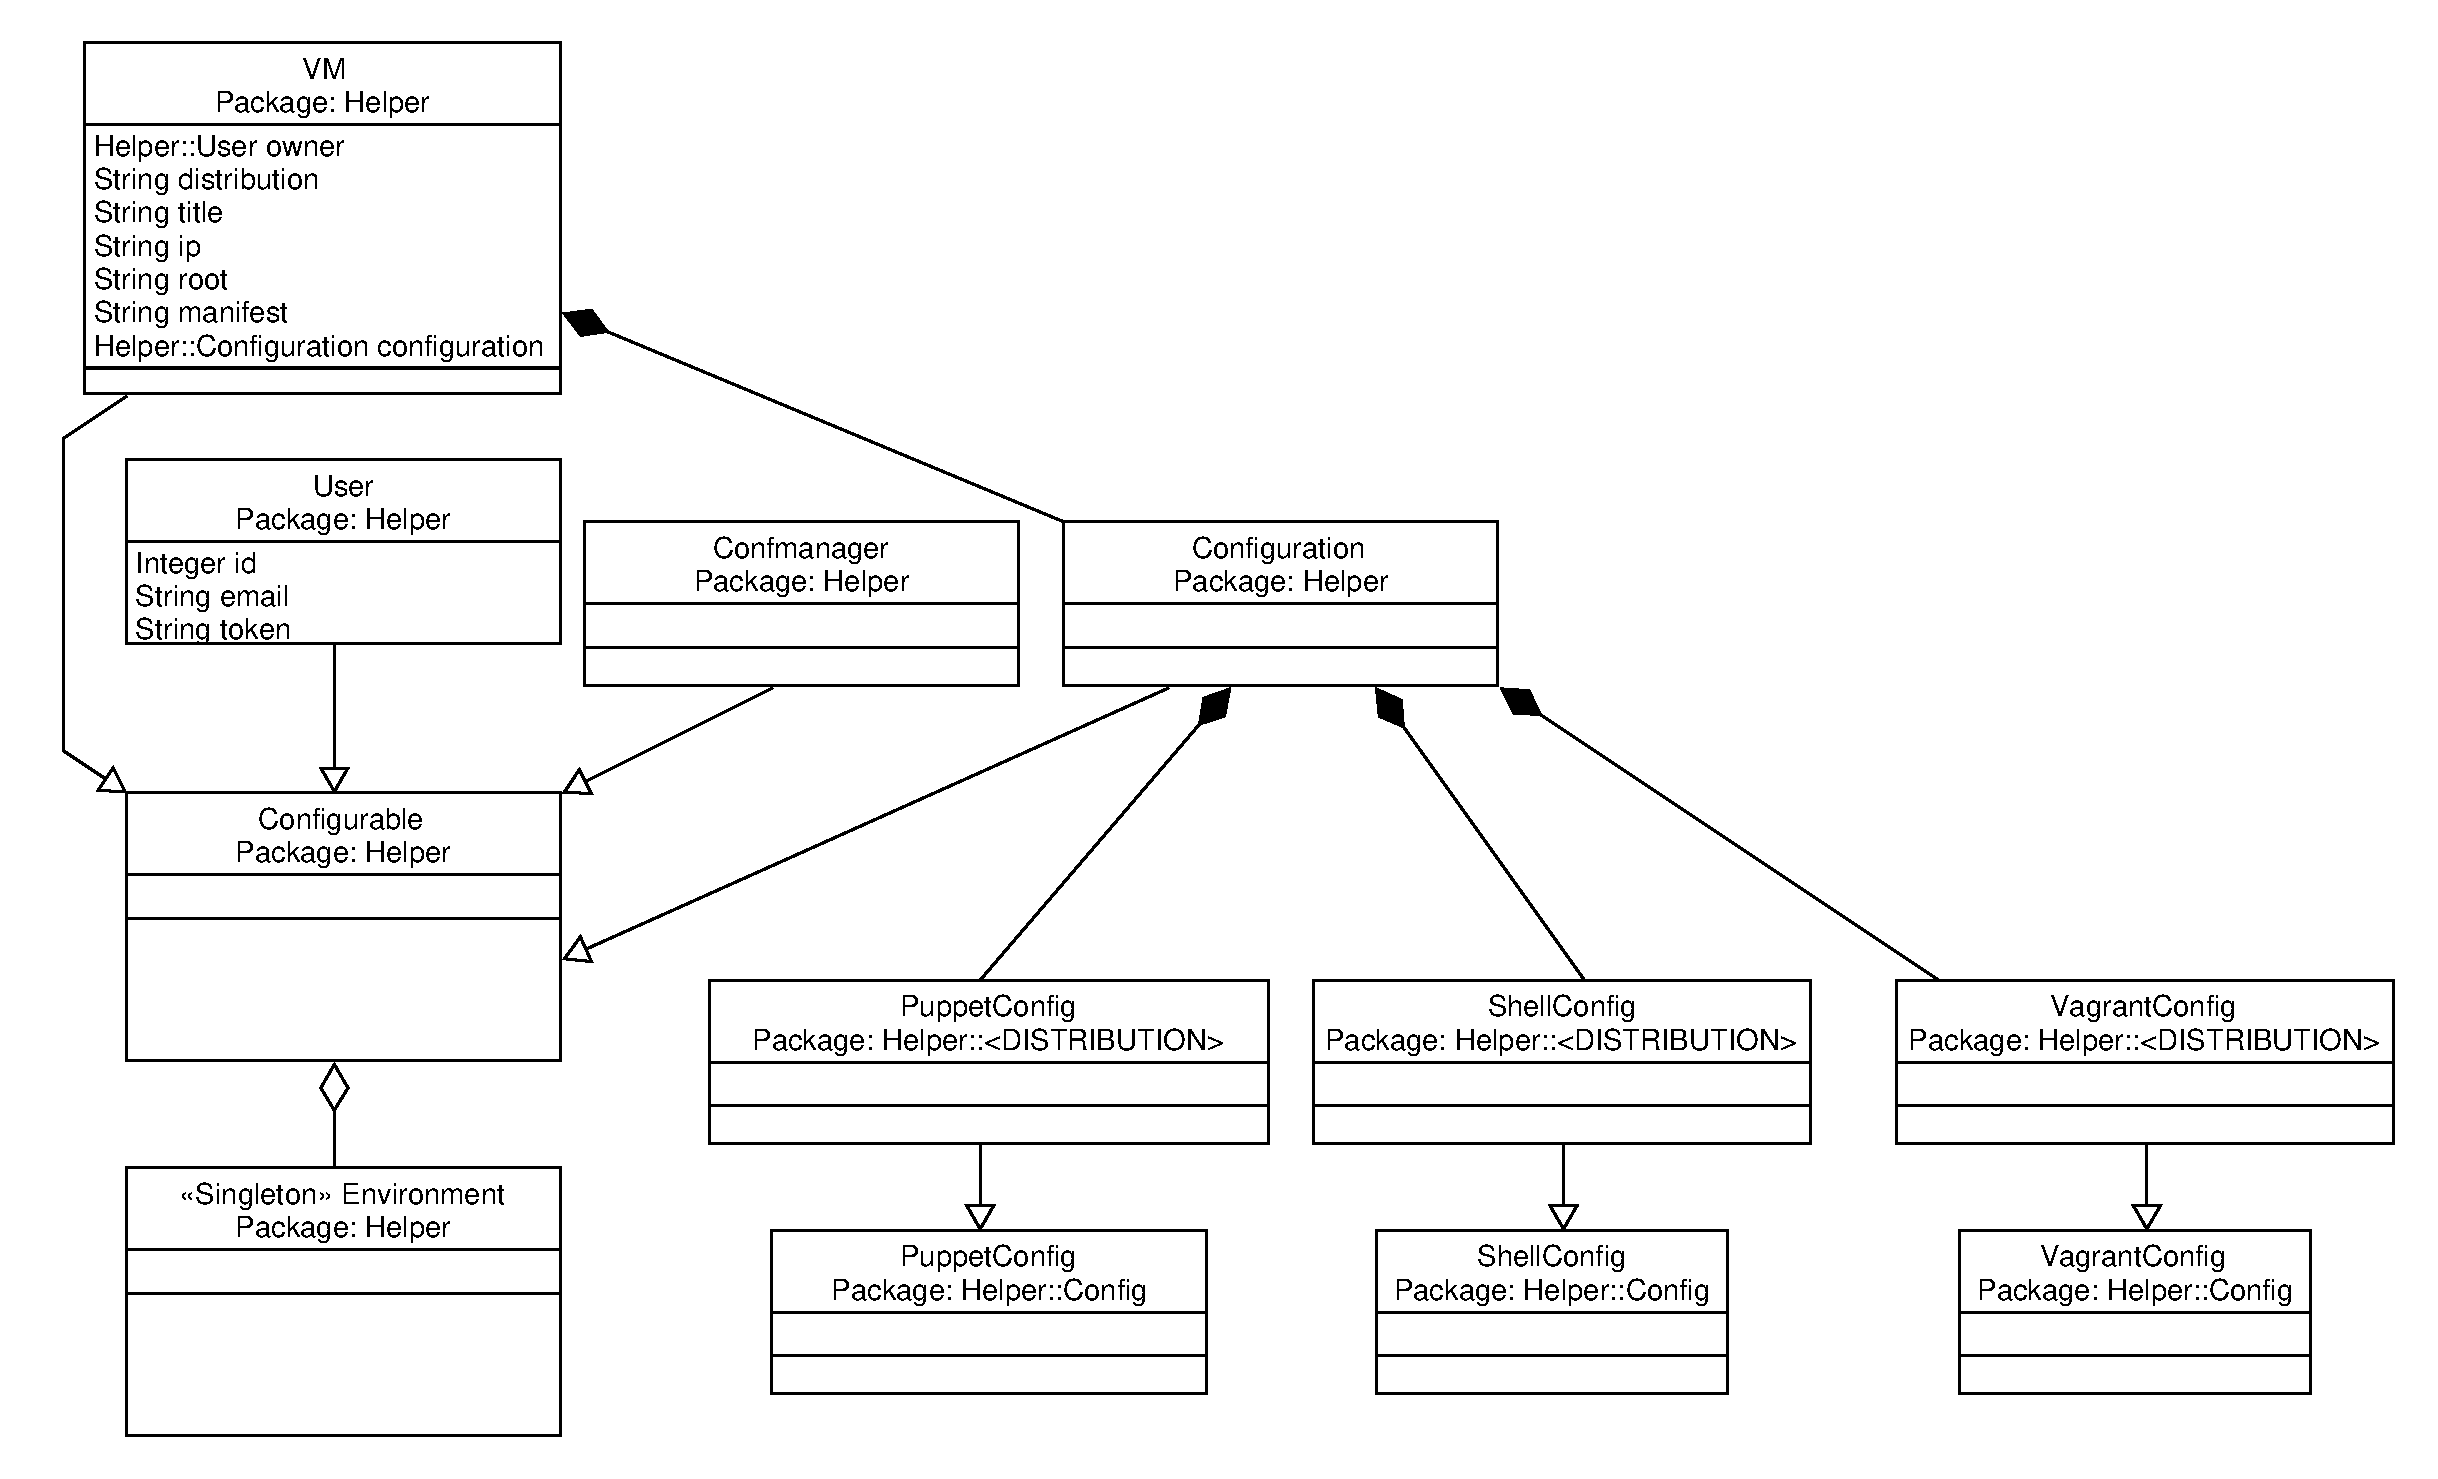
\includepdf{architecture.pdf}

\newpage
\section{Testing}

http://guides.rubygems.org/make-your-own-gem

\newpage
\section{Evaluation}

\newpage
\section{Conclusion}

\newpage
\section{References}
\bibliography{research}

\renewcommand{\bibname}{}

\newpage
\section{Glossary}
\printglossary
\newpage
\section{Appendix}


\begin{filecontents*}{research.bib}
	@online{a,
		author = {Internet Live Stats},
		title = {Google Search Statistics},
		url = {http://www.internetlivestats.com/google-search-statistics},
		urldate = {03.05.2014},
		note = {Accessed: November 26, 2016}
	},

	@online{b,
		author = {Techopedia Inc},
		title = {Definition of Virtualization},
		url = {https://www.techopedia.com/definition/719/virtualization},
		urldate = {2014},
		note = {Accessed: November 26, 2016}
	},

	@online{vagrant-definition,
		author = {Hashicorp},
		title = {WHY VAGRANT?},
		url = {https://www.vagrantup.com/docs/why-vagrant/},
		note = {Accessed: 27.03.2017}
	},

	@online{puppet-definition,
		author = {Puppet Labs},
		title = {Puppet Documentation},
		url = {https://docs.puppet.com/},
		note = {Accessed: 27.03.2017}
	},

	@online{ruby-on-rails-definition,
		author = {Ruby On Rails team},
		title = {Getting Started with Rails},
		url = {http://guides.rubyonrails.org/getting_started.html},
		note = {Accessed: 27.03.2017}
	},

	@online{ruby-definition,
		author = {Ruby team},
		title = {Ruby homepage},
		url = https://www.ruby-lang.org/en/},
	note = {Accessed: 27.03.2017}
	},


	@online{ictonline,
		author = {ITU ICT},
		title = {ICT Facts and Figures 2016},
		url = {http://www.itu.int/en/ITU-D/Statistics/Documents/facts/ICTFactsFigures2016.pdf},
		note = {Accessed: March 08, 2017}

	},

	@book{SecuringtheCloud,
		author    = {Vic (J.R.) Winkler},
		title     = {Securing the Cloud},
		year      = {2011},
		publisher = {Elsevier/Syngress},
	}

	@book{ibmvirtualisation,
		author    = {Shannon Meier},
		title     = {IBM Systems Virtualization: Servers, Storage, and Software},
		year      = {April 2008},
		publisher = {IBM},
	}

	@book{whatisnat,
		author    = {Javvin Technologies Inc},
		title     = {Network Protocols Handbook},
		year      = {2005},
		publisher = {Javvin Technologies},
	}


\end{filecontents*}

\bibliographystyle{plain}
\end{document}